\begin{appendix}
\twocolumn[{%
    \renewcommand\twocolumn[1][]{#1}%
    \begin{center}
        \centering
        \vskip -0.4cm
        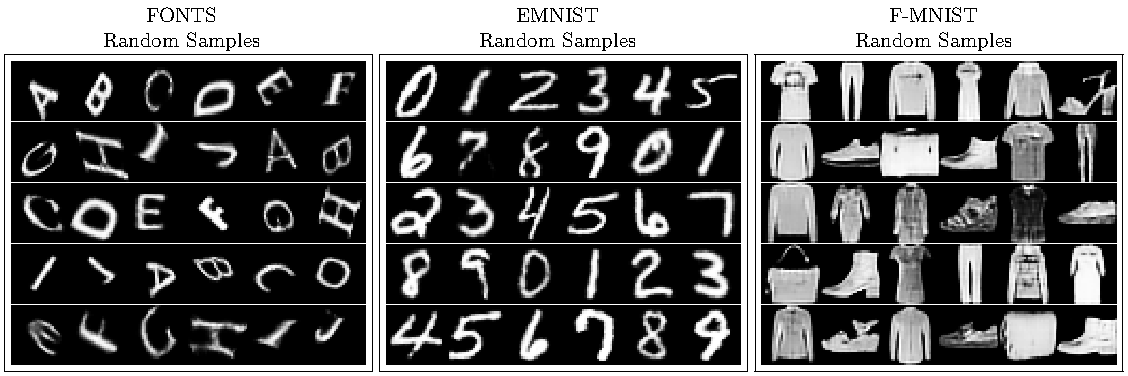
\includegraphics[width=\textwidth]{appendix_vaegan.pdf}
        \vskip -6px
        \captionof{figure}{
            For \Fonts (left), \MNIST (middle) and \Fashion (right), we show random samples from the learned, class-specific \VAEGANs used to craft on-manifold adversarial examples. Our \VAEGANs generate realistic looking samples; although we also include problematic samples illustrating the discrepancy between true and approximated data distribution.
        }
        \label{fig:appendix-vaegan}
        \vskip 24px
    \end{center}
}]

\section{Overview}

In the main paper, we study the relationship between adversarial robustness and generalization. Based on the distinction between regular and on-manifold adversarial examples, we show that
\begin{enumerate*}
	\item regular adversarial examples leave the underlying manifold of the data;
	\item on-manifold adversarial examples exist;
	\item on-manifold robustness is essentially generalization;
	\item and regular robustness is independent of generalization.
\end{enumerate*}
For clarity and brevity, the main paper focuses on the $L_{\infty}$ attack by Madry \etal \cite{MadryICLR2018} and the corresponding adversarial training variant applied to simple
convolutional neural networks. For on-manifold adversarial examples, we approximate the manifold using class-specific \VAEGANs \cite{LarsenICML2016,RoscaARXIV2017}. In this document, we present comprehensive experiments demonstrating that our findings generalize across attacks, adversarial training variants, network architectures and to class-agnostic \VAEGANs.

\subsection{Contents}

In \secref{sec:appendix-setup}, we present additional details regarding our experimental setup, corresponding to Section 3.1 of the main paper: in \secref{sec:appendix-fonts}, we discuss details of our synthetic \Fonts datasets and, in \secref{sec:appendix-vaegan}, we discuss our \VAEGAN implementation. Then, in \secref{sec:appendix-off-manifold} we extend the discussion of Section 3.2 with further results demonstrating that adversarial examples leave the manifold. Subsequently, in \secref{sec:appendix-on-manifold}, we show and discuss additional on-manifold adversarial examples to supplement the examples shown in Fig.\ 2 of the main paper. Then, complementing the discussion in Sections 3.4 and 3.5, we consider additional attacks, network architectures and class-agnostic \VAEGANs. Specifically, in \secref{sec:appendix-attacks}, we consider the $L_2$ variant of the white-box attack by Madry \etal \cite{MadryICLR2018}, the $L_2$ white-box attack by Carlini and Wagner \cite{CarliniSP2017}, and black-box transfer attacks. In \secref{sec:appendix-network}, we present experiments on multi-layer perceptrons and, in \secref{sec:appendix-data-manifold}, we consider approximating the manifold using class-agnostic \VAEGANs. In \secref{sec:appendix-adversarian-training}, corresponding to Section 3.6, we consider different variants of regular and on-manifold adversarial training. Finally, in \secref{sec:appendix-adversarial-example}, we discuss our definition of adversarial examples in the context of related work by Tsipras \etal \cite{TsiprasARXIV2018}, as outlined in Section 3.5.

\begin{figure*}[t]
    \centering
    \vskip -0.4cm
    \begin{subfigure}[t]{0.32\textwidth}
        \centering
        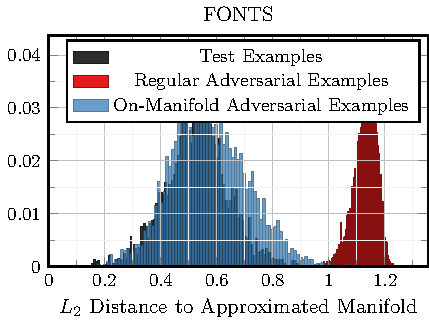
\includegraphics[width=1\textwidth]{appendix_manifold_a.pdf}
    \end{subfigure}
    \begin{subfigure}[t]{0.32\textwidth}
        \centering
        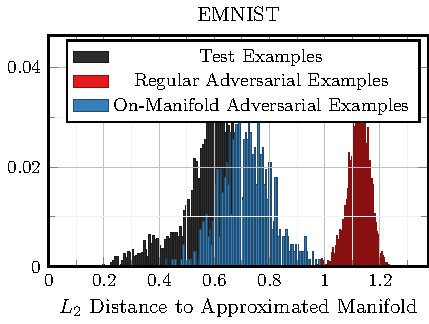
\includegraphics[width=1\textwidth]{appendix_manifold_c.pdf}
    \end{subfigure}
    \begin{subfigure}[t]{0.32\textwidth}
        \centering
        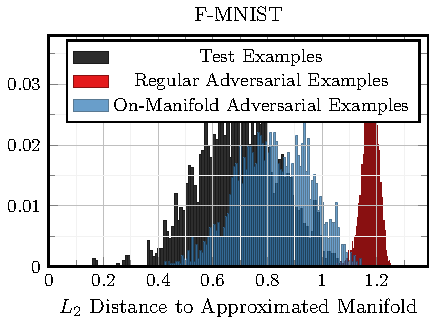
\includegraphics[width=1\textwidth]{appendix_manifold_b.pdf}
    \end{subfigure}
    \vskip -6px
    \caption{
        On \Fonts (left), \MNIST (middle) and \Fashion (right) we plot the distance of adversarial examples to the approximated manifold. We show normalized histograms of the $L_2$ distance of adversarial examples to their projection, as described in the text. Regular adversarial examples exhibit a significant distance to the manifold; clearly distinguishable from on-manifold adversarial examples and test images. We also note that, depending on the \VAEGAN approximation, on-manifold adversarial examples are hardly distinguishable from test images.
    }
    \label{fig:appendix-off-manifold}
\end{figure*}

\section{Experimental Setup}
\label{sec:appendix-setup}

We provide technical details on the introduced synthetic \Fonts dataset, \secref{sec:appendix-fonts}, and our \VAEGAN implementation, \secref{sec:appendix-vaegan}.

\subsection{\Fonts Dataset}
\label{sec:appendix-fonts}

Our \Fonts dataset consists of randomly rotated characters ``A'' to ``J'' from different fonts, as outlined in Section 3.1 of the main paper. Specifically, we consider $1000$ Google Fonts as downloaded from the corresponding GitHub repository\footnote{\url{https://github.com/google/fonts}}. We manually exclude fonts based on symbols, or fonts that could not be rendered correctly in order to obtain a cleaned dataset consisting of clearly readable letters ``A'' to ``J''; still, the $1000$ fonts exhibit significant variance. The obtained, rendered letters are transformed using translation, shear, scaling and rotation: for each letter and font, we create $112$ transformations, uniformly sampled in $[-0.2,0.2]$, $[-0.5, 0.5]$, $[0.75,1.15]$, and $[-\nicefrac{\pi}{2},\nicefrac{\pi}{2}]$, respectively. As a result, with $1000$ fonts and $10$ classes, we obtain $1.12\text{Mio}$ images of size $28{\times}28$, splitted into $960\text{k}$ training images and $160\text{k}$ test images (of which we use $40\text{k}$ in the main paper); thus, the dataset has four times the size of \MNIST \cite{CohenARXIV2017}. For simplicity, the transformations are applied using a spatial transformer network \cite{JaderbergNIPS2015} by assembling translation $[t_1, t_2]$, shear $[\lambda_1, \lambda_2]$, scale $s$ and rotation $r$ into an affine transformation matrix,
\vskip -14px
\begin{align}
    \hskip -4px
    \left[
        \begin{matrix}
            \cos(r) s - \sin(r) s \lambda_1 & -\sin(r) s + \cos(r) s \lambda_1 & t_1\\
            \cos(r) s \lambda_2 + \sin(r) s & -\sin(r) s \lambda_2 + \cos(r) s & t_2
        \end{matrix}
    \right],
\end{align}
\vskip -4px
\noindent making the generation process fully differentiable. Overall, \Fonts offers full control over the manifold, \ie, the transformation parameters, font and class, with differentiable generative model, \ie, decoder.

\subsection{VAE-GAN Variant}
\label{sec:appendix-vaegan}

As briefly outlined in Section 3.1 of the main paper, we use class-specific \VAEGANs \cite{LarsenICML2016,RoscaARXIV2017} to approximate the class-manifolds on all datasets, \ie, \Fonts, \MNIST \cite{CohenARXIV2017}, \Fashion \cite{XiaoARXIV2017} and \Celeb \cite{LiuICCV2015}. In contrast to \cite{LarsenICML2016}, however, we use a reconstruction loss on the image, not on the discriminator's features; in contrast to \cite{RoscaARXIV2017}, we use the standard Kullback-Leibler divergence to regularize the latent space. The model consists of an encoder $\enc$, approximating the posterior $q(z|x) \approx p(z|x)$ of latent code $z$ given image $x$, a (deterministic) decoder $\dec$, and a discriminator $\dis$. During training, the sum of the following losses is minimized:
\vskip -14px
\begin{align}
    &\cL_{\enc} = \mE_{q(z|x)}\left[\lambda\|x - \dec(z)\|_1\right] + \text{KL}(q(z|x)|p(z))\label{eq:appendix-vaegan-1}\\
    &\cL_{\dec} = \mE_{q(z|x)}\left[\lambda\|x - \dec(z)\|_1 - \log(\dis(\dec(z))) \right]\label{eq:appendix-vaegan-2}\\
    &\begin{aligned}
        \cL_{\dis} = &- \mE_{p(x)}\left[\log(\dis(x))\right]\\
        &- \mE_{q(z|x)}\left[\log(1 - \dis(\dec(z)))\right]\label{eq:appendix-vaegan-3}
    \end{aligned}
\end{align}
\vskip -4px
\noindent using a standard Gaussian prior $p(z)$. Here, $q(z|x)$ is modeled by predicting the mean $\mu(x)$ and variance $\sigma^2(x)$ such that $q(z|x) = \mathcal{N}(z; \mu(x), \text{diag}(\sigma^2(x)))$ and the weighting parameter $\lambda$ controls the importance of the $L_1$ reconstruction loss relative to the Kullback-Leibler divergence $\text{KL}$ and the adversarial loss for decoder and discriminator. As in~\cite{KingmaICLR2014}, we use the reparameterization trick with one sample to approximate the expectations in \eqnref{eq:appendix-vaegan-1}, \eqref{eq:appendix-vaegan-2} and \eqref{eq:appendix-vaegan-3}, and the Kullback-Leibler divergence $\text{KL}(q(z|x)|p(z))$ is computed analytically.

The encoder, decoder and discriminator consist of three (four for \Celeb) (de-) convolutional layers ($4{\times}4$ kernels; stride $2$; $64$, $128$, $256$ channels), followed by ReLU activations and batch normalization \cite{IoffeICML2015}; the encoder uses two fully connected layers to predict mean and variance; the discriminator uses two fully connected layers to predict logits. We tuned $\lambda$ to dataset- and class-specific values: on \Fonts, $\lambda = 3$ worked well for all classes, on \MNIST, $\lambda = 2.5$ except for classes ``0'' ($\lambda = 2.75$), ``1'' ($\lambda = 5.6$) and ``8'' ($\lambda = 2.25$), on \Fashion, $\lambda = 2.75$ worked well for all classes, on \Celeb $\lambda = 3$ worked well for both classes. Finally, we trained our \VAEGANs using ADAM~\cite{KingmaICLR2015} with learning rate $0.005$ (decayed by $0.9$ every epoch), weight decay $0.0001$ and batch size $100$ for $10$, $30$, $60$ and $30$ epochs on \Fonts, \MNIST, \Fashion and \Celeb, respectively. We also consider class-agnostic \VAEGANs trained using the same strategy with $\lambda = 3$ for \Fonts, $\lambda = 3$ on \MNIST, $\lambda =2.75$ on \Fashion and $\lambda=3$ on \Celeb, see \secref{sec:appendix-data-manifold} for results.

In \figref{fig:appendix-vaegan}, we include random samples of the class-specific \VAEGANs. Especially on \MNIST and \Fonts, our \VAEGANs generate realistic looking samples with sharp edges. However, we also show several problematic random samples, illustrating the discrepancy between the true data distribution and the approximation -- as particularly highlighted on \Fonts.

\section{Adversarial Example Distance to Manifold}
\label{sec:appendix-off-manifold}

Complementing Section 3.2 of the main paper, we provide additional details and results regarding the distance of regular adversarial examples to the true or approximated manifold, \red{including a theoretical argument of adversarial examples leaving the manifold}.

\begin{figure*}[t]
    \centering
    \vskip -0.4cm
    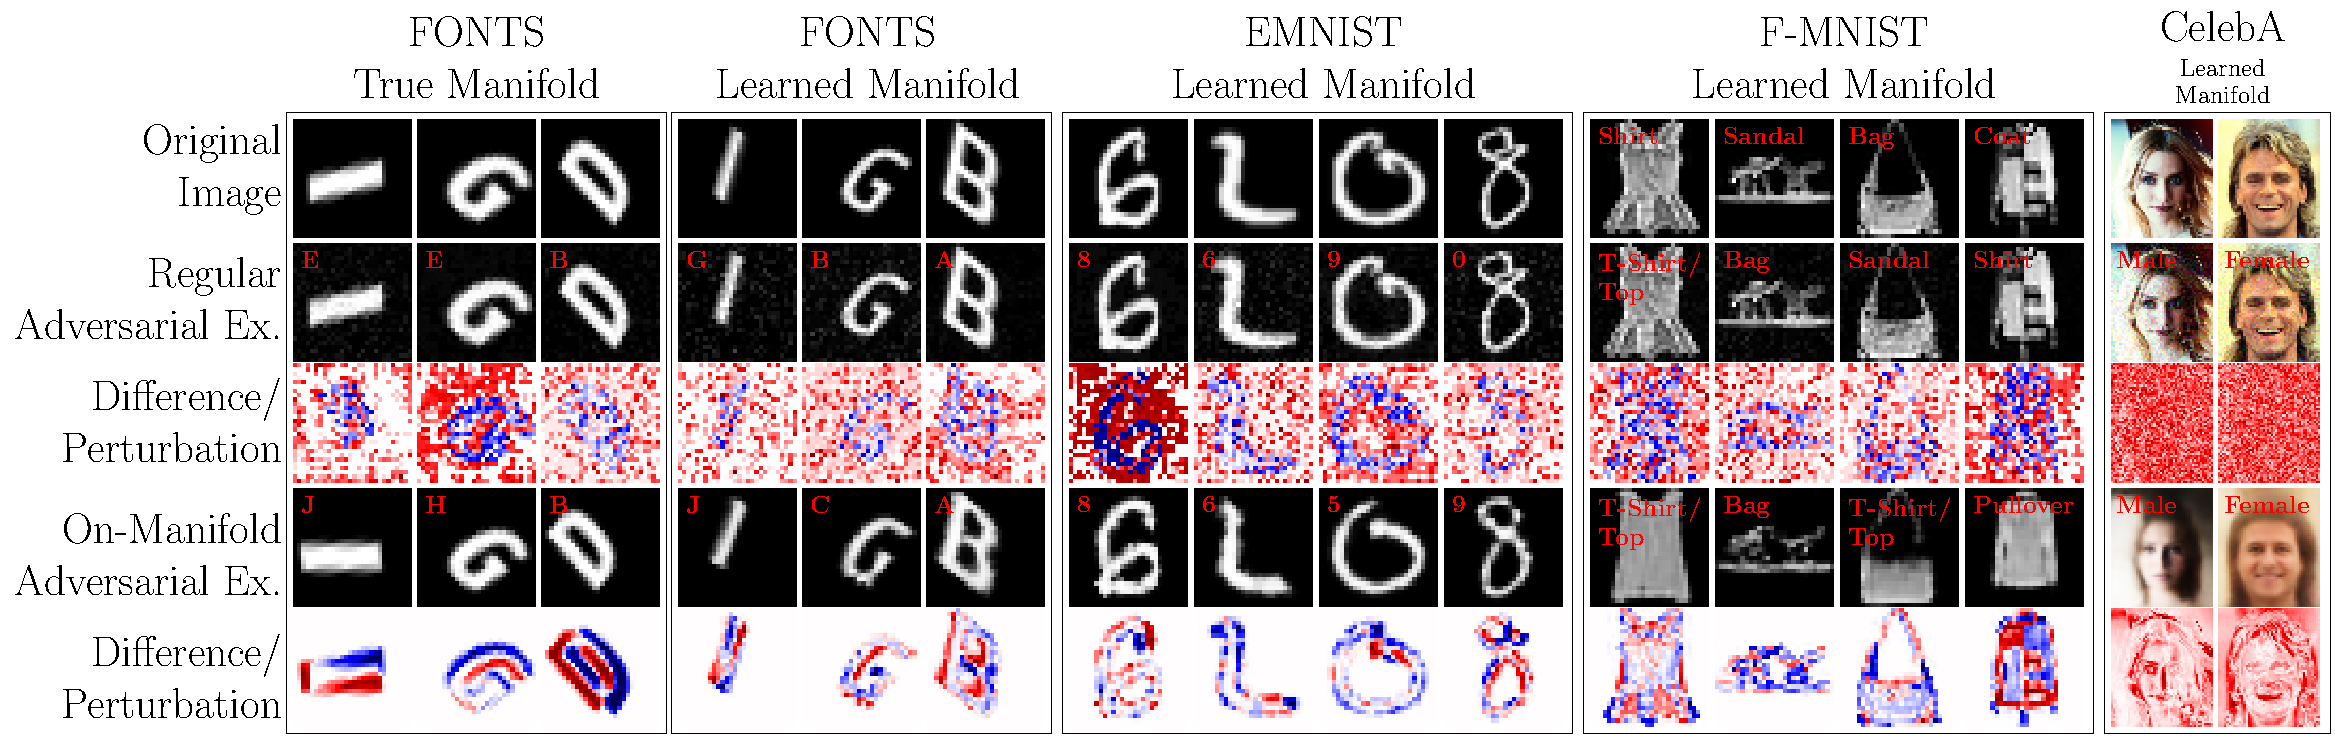
\includegraphics[width=1\textwidth]{appendix_examples.pdf}
    \vskip -6px 
    \caption{Regular and on-manifold adversarial examples on \Fonts, \MNIST, \Fashion and \Celeb. On \Fonts, the manifold is known; on the other datasets, class manifolds have been approximated using \VAEGANs. Notice that the crafted on-manifold adversarial examples correspond to meaningful manipulations of the image -- as long as the learned class-manifolds are good approximations. This can best be seen considering the (normalized) difference images (or the magnitude thereof for \Celeb).}
    \label{fig:appendix-examples}
\end{figure*}

On \Fonts, with access to the true manifold in form of a perfect decoder $\dec$, we iteratively obtain the latent code $\tilde{z}$ yielding the manifold's closest image to the given adversarial example $\tilde{x}$ as
\vskip -14px
\begin{align}
    \tilde{z} = \argmin_z \|\tilde{x} - \dec(z)\|_2^2.
\end{align}
\vskip -4px
\noindent We use $100$ iterations of ADAM \cite{KingmaICLR2015}, with a learning rate of $0.09$, decayed every $10$ iterations by a factor $0.95$. We found that additional iterations did not improve the results. The obtained projection $\pi(\tilde{x}) = \dec(\tilde{z})$ is usually very close to the original test image $x$ for which the adversarial example was crafted. The distance is then computed as $\|\tilde{x} - \pi(\tilde{x})\|_2$; we refer to the main paper for results and discussion.

If the true manifold is not available, we locally approximate the manifold using $50$ nearest neighbors $x_1,\ldots,x_{50}$ of the adversarial example $\tilde{x}$. In the main paper, we center these nearest neighbors at the test image $x$, \ie, consider the sub-space spanned by $x_i - x$. Here, we show that the results can be confirmed when centering the nearest neighbors at their mean $\bar{x} = \nicefrac{1}{50} \sum_{i = 1}^{50} x_i$ and considering the subspace spanned by $x_i - \bar{x}$ instead. In this scenario, the test image $x$ is not necessarily part of the approximated manifold anymore. The projection onto this sub-space can be obtained by solving the least squares problem; specifically, we consider the vector $\delta = \tilde{x} - x$, \ie, we assume that the ``adversarial direction'' originates at the mean $\bar{x}$. Then, we solve
\vskip -14px
\begin{align}
    \beta^\ast = \argmin_\beta \|X\beta - \delta\|_2^2\label{eq:appendix-least-squares}
\end{align}
\vskip -4px
\noindent where the columns $X_i$ are the vectors $x_i - \bar{x}$. The projection $\pi(\tilde{x})$ is obtained as $\pi(\tilde{x}) = X\beta^\ast$; the same approach can be applied to projecting the test image $x$. Note that it is crucial to consider the adversarial direction $\delta$ itself, instead of the adversarial example~$\tilde{x}$ because $\|\delta\|_2$ is small by construction, \ie, the projections of $\tilde{x}$ and $x$ are very close. In \figref{fig:appendix-off-manifold}, we show results using this approximation on \Fonts, \MNIST and \Fashion. Regular adversarial examples can clearly be distinguished from test images and on-manifold adversarial examples. Note, however, that we assume access to both the test image $x$ and the corresponding adversarial example $\tilde{x}$ such that this finding cannot be exploited for detection. We also notice that the discrepancy between the distance distributions of test images and on-manifold adversarial examples reflects the approximation quality of the used \VAEGANs.

\subsection{Intuition and Theoretical Argument}

\red{Having empirically shown that regular adversarial examples tend to leave the manifold, often in a nearly orthogonal direction, we also discuss a theoretical argument supporting this observation. The main assumption is that the training loss is constant on the manifold (normally close to zero) due to training and proper generalization, \ie, low training and test loss. Thus, the loss gradient is approximately orthogonal to the manifold as this is the direction to increase the loss most efficiently.}

\begin{figure*}[t]
    \centering
    \vskip -0.4cm
    \begin{subfigure}{0.255\textwidth}
        \centering
        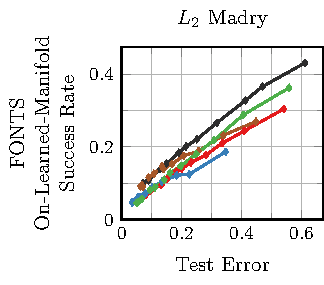
\includegraphics[width=\textwidth]{appendix_l2_fonts_error_on_learned_madry.pdf}
    \end{subfigure}
    \begin{subfigure}{0.235\textwidth}
        \centering
        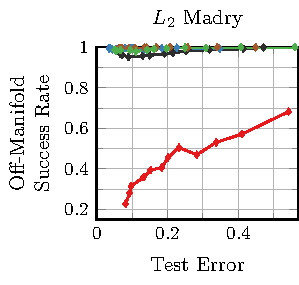
\includegraphics[width=\textwidth]{appendix_l2_fonts_error_off_madry.pdf}
    \end{subfigure}
    \begin{subfigure}{0.235\textwidth}
        \centering
        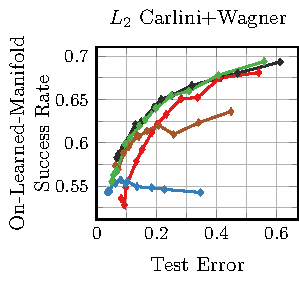
\includegraphics[width=\textwidth]{appendix_l2_fonts_error_on_learned_cw.pdf}
    \end{subfigure}
    \begin{subfigure}{0.235\textwidth}
        \centering
        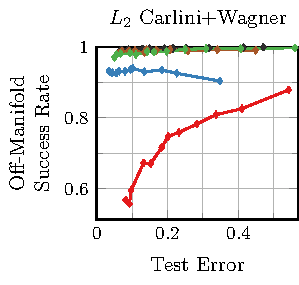
\includegraphics[width=\textwidth]{appendix_l2_fonts_error_off_cw.pdf}
    \end{subfigure}
    \\
    \begin{subfigure}{0.255\textwidth}
        \centering
        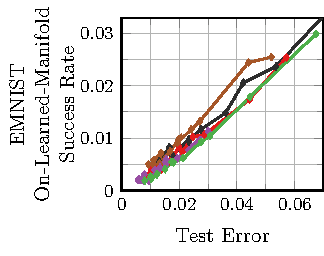
\includegraphics[width=\textwidth]{appendix_l2_emnist_error_on_learned_madry.pdf}
    \end{subfigure}
    \begin{subfigure}{0.235\textwidth}
        \centering
        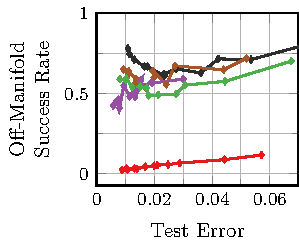
\includegraphics[width=\textwidth]{appendix_l2_emnist_error_off_madry.pdf}
    \end{subfigure}
    \begin{subfigure}{0.235\textwidth}
        \centering
        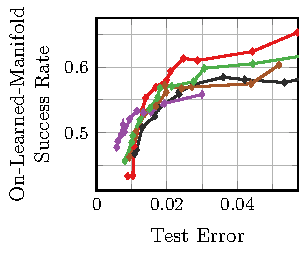
\includegraphics[width=\textwidth]{appendix_l2_emnist_error_on_learned_cw.pdf}
    \end{subfigure}
    \begin{subfigure}{0.235\textwidth}
        \centering
        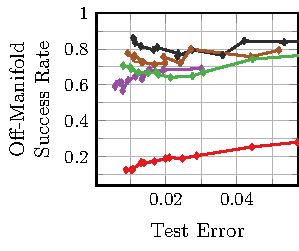
\includegraphics[width=\textwidth]{appendix_l2_emnist_error_off_cw.pdf}
    \end{subfigure}
    \\
    \begin{subfigure}{0.255\textwidth}
        \centering
        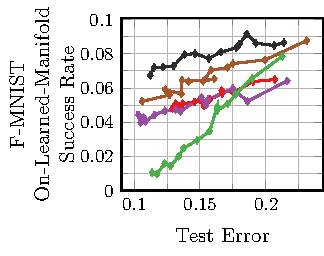
\includegraphics[width=\textwidth]{appendix_l2_fashion_error_on_learned_madry.pdf}
    \end{subfigure}
    \begin{subfigure}{0.235\textwidth}
        \centering
        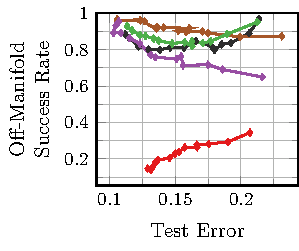
\includegraphics[width=\textwidth]{appendix_l2_fashion_error_off_madry.pdf}
    \end{subfigure}
    \begin{subfigure}{0.235\textwidth}
        \centering
        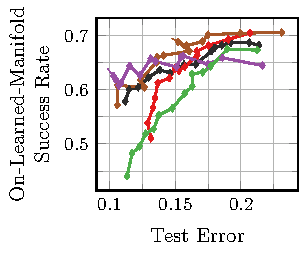
\includegraphics[width=\textwidth]{appendix_l2_fashion_error_on_learned_cw.pdf}
    \end{subfigure}
    \begin{subfigure}{0.235\textwidth}
        \centering
        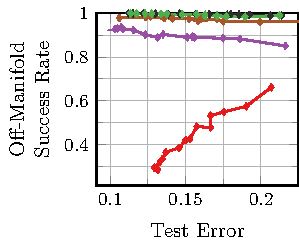
\includegraphics[width=\textwidth]{appendix_l2_fashion_error_off_cw.pdf}
    \end{subfigure}
    \\
    \fcolorbox{black!50}{white}{
        \begin{subfigure}{1\textwidth}
            \centering
            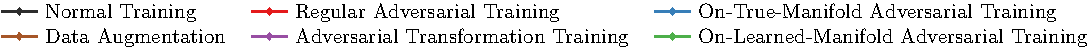
\includegraphics[width=0.825\textwidth]{appendix_l2_legend.pdf}
        \end{subfigure}
    }
    \caption{
        $L_2$ attacks of Madry \etal \cite{MadryICLR2018} and Carlini and Wagner \cite{CarliniSP2017} on \Fonts, \MNIST and \Fashion. In all cases, we plot regular or on-manifold success rate against test error. Independent of the attack, we can confirm that on-manifold robustness is strongly related to generalization, while regular robustness is independent of generalization.
    }
    \label{fig:appendix-l2}
\end{figure*}

\red{More formally, let $f(x)$ denote the classifier which -- for simplicity -- takes inputs $x \in \mathbb{R}^d$ and predicts outputs $y \in \mathbb{R}^K$ for $K$ classes. We assume both the classifier as well as the used loss, \eg, cross-entropy loss, to be differentiable. We further expect the data to lie on a manifold $\mathcal{M}$ and the loss to be constant on $\mathcal{M} \cap B(x, \epsilon)$ with 
\begin{align}
    B(x, \epsilon) = \{x' \in \mathbb{R}^d: \|x' - x\| \leq \epsilon\}.
\end{align}
Let
\begin{align}
    g(x) = \mathbb{E}\left[ \cL(f(x), y)|x\right]
\end{align}
be the conditional expectation of the loss $\cL$; then, by the mean value theorem, there exists $\theta(x') \in [0,1]$ for each $x' \in \mathcal{M} \cap B(x, \epsilon)$ such that
\begin{align}
    0 &= g(x') - g(x)\\
    &= \inner{\nabla g(\theta(x') x + (1 - \theta(x'))x'), x' - x}
\end{align}
As this holds for all $\epsilon > 0$ and as $\epsilon \rightarrow 0$, every vector $x' - x$ becomes a tangent of $\mathcal{M}$ at $x$ and
\begin{align}
    \lim_{\epsilon \rightarrow 0} \nabla g(\theta(x') x + (1 - \theta(x'))x') = \nabla g(x),
\end{align}
it holds that $\nabla g(x)$ is orthogonal to the tangent space of $\mathcal{M}$ at $x$. As $\nabla g(x)$ is the gradient of the expected loss, it implies that adversarial examples, as computed, \eg, using first-order gradient-based approaches such as \eqnref{eq:appendix-off-manifold-madry}, leave the manifold $\mathcal{M}$ in order to fool the classifier $f(x)$.}

\section{On-Manifold Adversarial Examples}
\label{sec:appendix-on-manifold}

In \figref{fig:appendix-examples}, we show additional examples of regular and on-manifold adversarial examples, complementing the examples in Fig.\ 2 of the main paper. On \Fonts, both using the true and the approximated manifold, on-manifold adversarial examples reflect the underlying invariances of the data, \ie, the transformations employed in the generation process. This is in contrast to the corresponding regular adversarial examples and their (seemingly) random noise patterns. We note that regular and on-manifold adversarial examples can best be distinguished based on their difference to the original test image -- although both are perceptually close to the original image. Similar observations hold on \MNIST and \Fashion. However, especially on \Fashion and \Celeb, the discrepancy between true images and on-manifold adversarial examples becomes visible. This is the ``cost'' of approximating the underlying manifold using \VAEGANs. More examples can be found in \figref{fig:appendix-examples-2} at the end of this document.

\section{$L_2$ and Transfer Attacks}
\label{sec:appendix-attacks}

\begin{figure}[t]
    \centering
    \vskip -0.4cm
    \begin{subfigure}{0.245\textwidth}
        \centering
        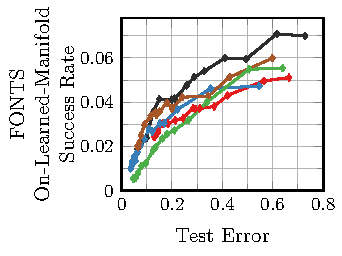
\includegraphics[width=\textwidth]{appendix_transfer_fonts_error_on_learned.pdf}
    \end{subfigure}
    \begin{subfigure}{0.225\textwidth}
        \centering
        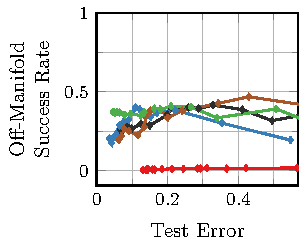
\includegraphics[width=\textwidth]{appendix_transfer_fonts_error_off.pdf}
    \end{subfigure}
    \\
    \begin{subfigure}{0.245\textwidth}
        \centering
        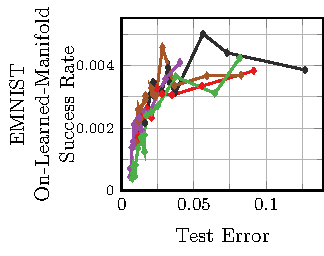
\includegraphics[width=\textwidth]{appendix_transfer_emnist_error_on_learned.pdf}
    \end{subfigure}
    \begin{subfigure}{0.225\textwidth}
        \centering
        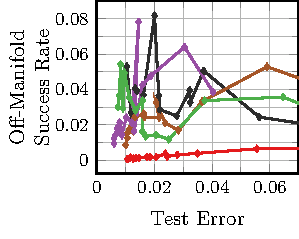
\includegraphics[width=\textwidth]{appendix_transfer_emnist_error_off.pdf}
    \end{subfigure}
    \\
    \begin{subfigure}{0.245\textwidth}
        \centering
        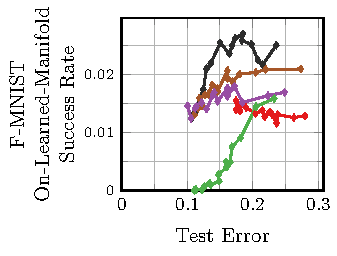
\includegraphics[width=\textwidth]{appendix_transfer_fashion_error_on_learned.pdf}
    \end{subfigure}
    \begin{subfigure}{0.225\textwidth}
        \centering
        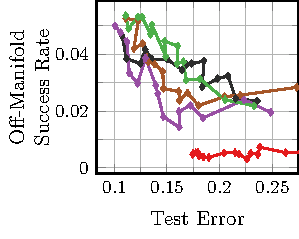
\includegraphics[width=\textwidth]{appendix_transfer_fashion_error_off.pdf}
    \end{subfigure}
    \\
    \fcolorbox{black!50}{white}{
        \begin{subfigure}{0.45\textwidth}
            \centering
            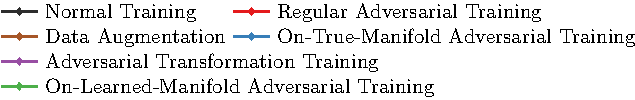
\includegraphics[width=1\textwidth]{appendix_transfer_legend.pdf}
        \end{subfigure}
    }
    \caption{Transfer attacks on \Fonts, \MNIST and \Fashion. We show on-manifold (left) and regular success rate (right) plotted against test error. In spite of significantly lower success rates, transfer attacks also allow to confirm the strong relationship between on-manifold success rate and test error, while -- at least on \Fonts and \MNIST -- regular success rate is independent of test error.}
    \label{fig:appendix-transfer}
\end{figure}

In the main paper, see Section 3.1, we primarily focus on the $L_{\infty}$ white-box attack by Madry \etal \cite{MadryICLR2018}. Here, we further consider the $L_2$ variant, which, given image $x$ with label $y$ and classifier $f$, maximizes the training loss, \ie,
\vskip -14px
\begin{align}
    \max_\delta \cL(f(x + \delta), y)\text{ s.t. }\|\delta\|_2 \leq \epsilon, \tilde{x}_i \in [0,1],
    \label{eq:appendix-off-manifold-madry}
\end{align}
\vskip -4px
\noindent to obtain an adversarial example $\tilde{x} = x + \delta$. \red{We use $\epsilon = 1.5$ for regular adversarial examples and $\epsilon = 0.3$ for on-manifold adversarial examples. For optimization, we utilize} projected ADAM \cite{KingmaICLR2015}: after each iteration, $\tilde{x}$ is projected onto the $L_2$-ball of radius $\epsilon$ using 
\vskip -14px
\begin{align}
    \tilde{x}' = \tilde{x} \cdot \max\left(1, \frac{\epsilon}{\|\tilde{x}\|_2}\right)
\end{align}
\vskip -4px
\noindent and clipped to $[0, 1]$. We use a learning rate of $0.005$ and we note that ADAM includes momentum, as suggested in~\cite{DongCVPR2018}. Optimization stops as soon as the label changes, or runs for a maximum of $40$ iterations. The perturbation $\delta$ is initialized randomly as follows:
\vskip -14px
\begin{align}
    \delta = u \epsilon \frac{\delta'}{\|\delta'\|_2},\quad \delta' \sim \mathcal{N}(0, I), u \sim U(0,1).
\end{align}
\vskip -4px
\noindent Here, $U(0,1)$ refers to the uniform distribution over $[0,1]$. This results in $\delta$ being in the $\epsilon$-ball and uniformly distributed over distance and direction. Note that this is in contrast to sampling uniformly \wrt the volume of the $\epsilon$-ball. The same procedure applies to the $L_{\infty}$ attack where the projection onto the $\epsilon$-ball is achieved by clipping. The attack can also be used to obtain on-manifold adversarial examples, as described in Section 3.3 of the main paper. Then, optimization in \eqnref{eq:appendix-off-manifold-madry} is done over the perturbation $\zeta$ in latent space, with constraint $\|\zeta\|_2 \leq \eta$. The adversarial example is obtained as $\tilde{x} = \dec(z + \zeta)$ with $z$ being the latent code of image $x$ and $\dec$ being the true or approximated generative model, \ie, decoder.

\begin{figure}[t]
    \centering
    \vskip -0.4cm
    \hskip -0.1cm
    \begin{subfigure}[t]{0.5\textwidth}
        \begin{subfigure}[t]{0.49\textwidth}
            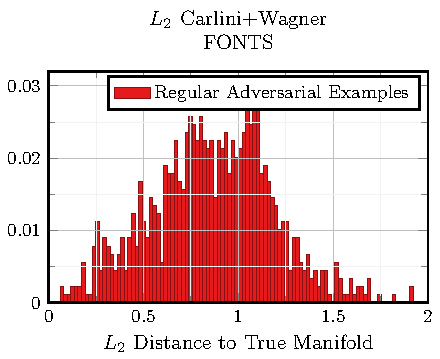
\includegraphics[width=0.9\textwidth]{appendix_manifold_d.pdf}
        \end{subfigure}
        \begin{subfigure}[t]{0.49\textwidth}
            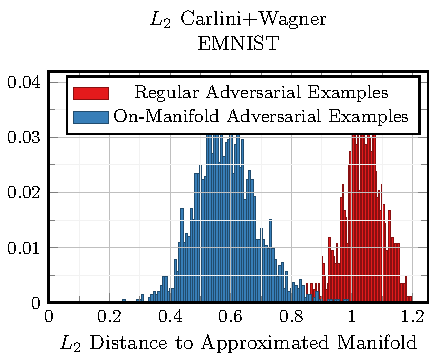
\includegraphics[width=0.9\textwidth]{appendix_manifold_e.pdf}
        \end{subfigure}
    \end{subfigure}
    \vskip -6px
    \caption{\red{Distance of Carlini+Wagner adversarial examples to the true, on \Fonts (left), or approximated, on \MNIST (right), manifold. As before, we show normalized histograms of the $L_2$ distance of adversarial examples to their projections onto the manifold. Even for different attacks and the $L_2$ norm, regular adversarial examples seem to leave the manifold.}}
    \label{fig:appendix-off-manifold-cw}
\end{figure}

We also consider the $L_2$ white box attack by Carlini and Wagner \cite{CarliniSP2017}. Instead of directly maximizing the training loss, Carlini and Wagner propose to use a surrogate objective on the classifier's logits $l_y$:
\vskip -14px
\begin{align}
    F(\tilde{x}, y) &= \max(-\kappa, l_y(\tilde{x}) - \max_{y' \neq y} l_{y'}(\tilde{x})).
\end{align}
\vskip -4px
\noindent Compared to the training loss, which might be close to zero for a well-trained network, $F$ is argued to provide more useful gradients \cite{CarliniSP2017}. Then,
\vskip -14px
\begin{align}
    \min_\delta F(x + \delta, y) + \lambda \|\delta\|_2\text{ s.t. }\tilde{x}_i \in [0,1]
\end{align}
\vskip -4px
\noindent is minimized by reparameterizing $\delta$ in terms of $\delta= \nicefrac{1}{2}(\tanh(\omega) + 1)- x$ in order to ensure the image-constraint, \ie, $\tilde{x}_i \in [0,1]$. In practice, we empirically chose $\kappa = 1.5$, use $120$ iterations of ADAM \cite{KingmaICLR2015} with learning rate $0.005$ and $\lambda = 1$. Again, this attack can be used to obtain on-manifold adversarial examples, as well.

As black-box attack we transfer $L_\infty$ Madry adversarial examples from a held out model, as previously done in \cite{LiuICLR2017,XieARXIV2018,PapernotASIACCS2017}. The held out transfer model is trained normally, \ie, without any data augmentation or adversarial training, on $10\text{k}$ training images for $20$ epochs (as outlined in Section 3.1 of the main paper). The success rate of these transfer attacks is computed with respect to images that are correctly classified by both the transfer model and the target model.

Extending the discussion of Sections 3.4 and 3.5 of the main paper, \figref{fig:appendix-l2} shows results on \Fonts, \MNIST and \Fashion considering both $L_2$ attacks, \ie, Madry \etal \cite{MadryICLR2018} and Carlini and Wagner \cite{CarliniSP2017}. In contrast to the $L_{\infty}$ Madry attack, we observe generally lower success rates. Nevertheless, we can observe a clear relationship between on-manifold success rate and test error. The exact form of this relationship, however, depends on the attack; for the $L_2$ Madry attack, the relationships seems to be mostly linear (especially on \Fonts and \MNIST), while it seems non-linear for the $L_2$ Carlini and Wagner attack. Furthermore, the independence of regular robustness and generalization can be confirmed, \ie, regular success rate is roughly constant when test error varies -- again, with the exception of regular adversarial training. \red{Finally, for completeness, in \figref{fig:appendix-off-manifold-cw}, we illustrate that the Carlini+Wagner $L_2$ attack also results in regular adversarial examples leaving the manifold.}

\begin{figure}[t]
    \centering
    \vskip -0.4cm
    \begin{subfigure}{0.245\textwidth}
        \centering
        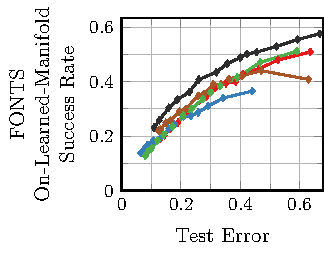
\includegraphics[width=\textwidth]{appendix_mlp_fonts_error_on_learned.pdf}
    \end{subfigure}
    \begin{subfigure}{0.225\textwidth}
        \centering
        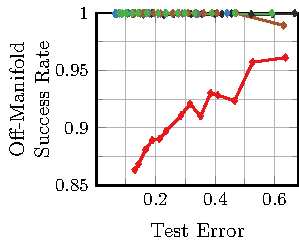
\includegraphics[width=\textwidth]{appendix_mlp_fonts_error_off.pdf}
    \end{subfigure}
    \\
    \begin{subfigure}{0.245\textwidth}
        \centering
        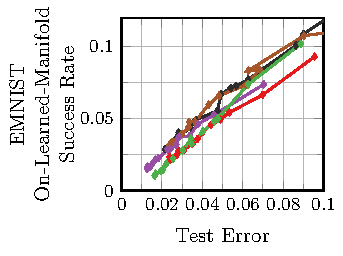
\includegraphics[width=\textwidth]{appendix_mlp_emnist_error_on_learned.pdf}
    \end{subfigure}
    \begin{subfigure}{0.225\textwidth}
        \centering
        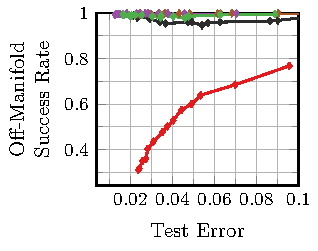
\includegraphics[width=0.925\textwidth]{appendix_mlp_emnist_error_off.pdf}
    \end{subfigure}
    \\
    \begin{subfigure}{0.245\textwidth}
        \centering
        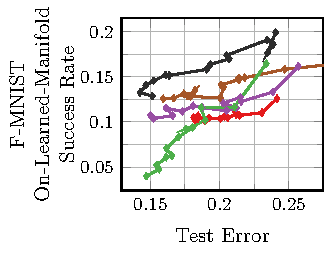
\includegraphics[width=\textwidth]{appendix_mlp_fashion_error_on_learned.pdf}
    \end{subfigure}
    \begin{subfigure}{0.225\textwidth}
        \centering
        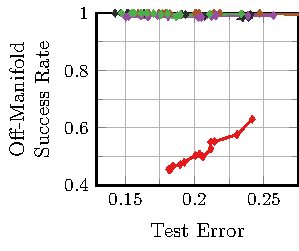
\includegraphics[width=0.925\textwidth]{appendix_mlp_fashion_error_off.pdf}
    \end{subfigure}
    \\
    \fcolorbox{black!50}{white}{
        \begin{subfigure}{0.45\textwidth}
            \centering
            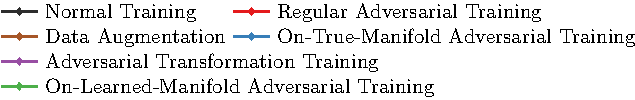
\includegraphics[width=1.01\textwidth]{appendix_mlp_legend.pdf}
        \end{subfigure}
    }
    \caption{Experiments with multilayer-perceptrons on \Fonts, \MNIST and \Fashion. We plot on-manifold (left) or regular success rate (right) against test error. On-manifold robustness is strongly related to generalization, while regular robustness seems mostly independent of generalization.}
    \label{fig:appendix-mlp}
\end{figure}
\begin{figure}
    \centering
    \vskip -0.4cm
    \begin{subfigure}{0.245\textwidth}
        \centering
        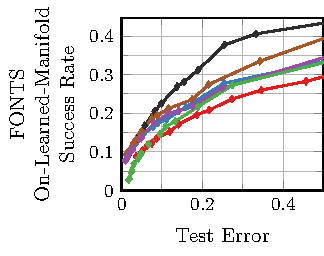
\includegraphics[width=\textwidth]{appendix_resnet_fonts_error_on_learned.pdf}
    \end{subfigure}
    \begin{subfigure}{0.225\textwidth}
        \centering
        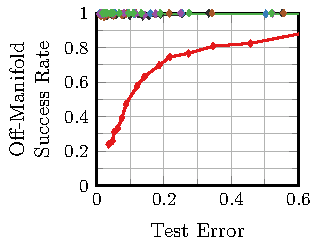
\includegraphics[width=\textwidth]{appendix_resnet_fonts_error_off.pdf}
    \end{subfigure}
    \\
    \begin{subfigure}{0.245\textwidth}
        \centering
        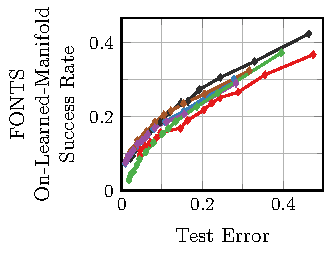
\includegraphics[width=\textwidth]{appendix_vgg2_fonts_error_on_learned.pdf}
    \end{subfigure}
    \begin{subfigure}{0.225\textwidth}
        \centering
        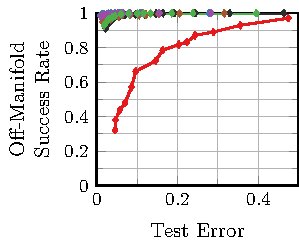
\includegraphics[width=0.925\textwidth]{appendix_vgg2_fonts_error_off.pdf}
    \end{subfigure}
    \\
    \begin{subfigure}{0.245\textwidth}
        \centering
        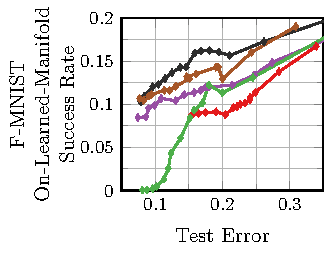
\includegraphics[width=\textwidth]{appendix_resnet_fashion_error_on_learned.pdf}
    \end{subfigure}
    \begin{subfigure}{0.225\textwidth}
        \centering
        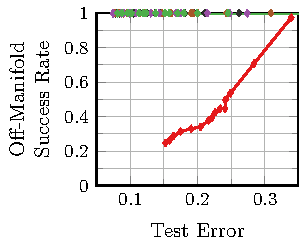
\includegraphics[width=\textwidth]{appendix_resnet_fashion_error_off.pdf}
    \end{subfigure}
    \\
    \begin{subfigure}{0.245\textwidth}
        \centering
        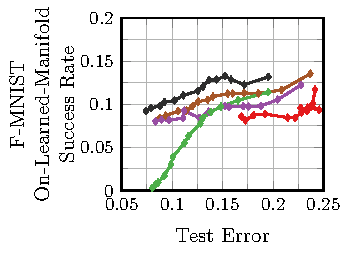
\includegraphics[width=\textwidth]{appendix_vgg_fashion_error_on_learned.pdf}
    \end{subfigure}
    \begin{subfigure}{0.225\textwidth}
        \centering
        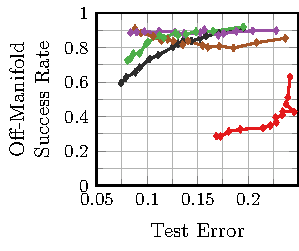
\includegraphics[width=0.925\textwidth]{appendix_vgg_fashion_error_off.pdf}
    \end{subfigure}
    \\
    \fcolorbox{black!50}{white}{
        \begin{subfigure}{0.45\textwidth}
            \centering
            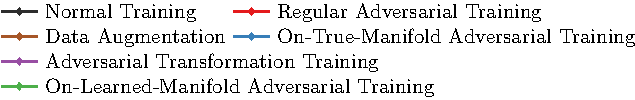
\includegraphics[width=1.01\textwidth]{appendix_mlp_legend.pdf}
        \end{subfigure}
    }
    \caption{\red{Experiments with ResNet-13 (top) and VGG (bottom) on \Fonts and \Fashion. We plot on-manifold (left) or regular success rate (right) against test error. As in \figref{fig:appendix-mlp}, our claims can be confirmed for these network architectures, as well.}}
    \label{fig:appendix-resnet-vgg}
\end{figure}

In \figref{fig:appendix-transfer}, we also consider the black-box case, \ie, without access to the target model. While both observations from above can be confirmed, especially on \Fonts and \MNIST, the results are significantly less pronounced. This is mainly due to the significantly lower success rate of transfer attacks -- both regarding regular and on-manifold adversarial examples. Especially on \MNIST and \Fashion, success rate may reduce from previously $80\%$ or higher to $10\%$ or lower. This might also explain the high variance on \MNIST and \Fashion regarding regular robustness. Overall, we demonstrate that our claims can be confirmed in both white- and black-box settings as well as using different attacks \cite{MadryICLR2018,CarliniSP2017} and norms.

\section{Influence of Network Architecture}
\label{sec:appendix-network}

Also in relation to the discussion in Sections 3.4 and 3.5 of the main paper, \figref{fig:appendix-mlp} shows results on \Fonts, \MNIST and \Fashion using multi-layer perceptrons instead of convolutional neural networks. Specifically, we consider a network with $4$ hidden layers, using $128$ hidden units each; each layer is followed by ReLU activations and batch normalization \cite{IoffeICML2015}; training strategy, however, remains unchanged. Both of our claims, \ie, that on-manifold robustness is essentially generalization but regular robustness is independent of generalization, can be confirmed. Especially regarding the latter, results are more pronounced using multi-layer perceptrons: except for regular adversarial training, success rate stays nearly constant at $100\%$ irrespective of test error. Overall, these results suggest that our claims generally hold for the class of (deep) neural networks, irrespective of architectural details.

\red{In order to further validate our claims, we also consider variants of two widely used, state-of-the-art architectures: ResNet-13 \cite{HeCVPR2016} and VGG \cite{SimonyanARXIV2014}. For VGG, however, we removed the included dropout layers. The main reason is that randomization might influence robustness, \eg, see \cite{AthalyeARXIV2018}. Additionally, we only use 2 stages of model A, see \cite{SimonyanARXIV2014}, in order to deal with the significantly lower resolution of $28 \times 28$ on \Fonts, \MNIST and \Fashion; finally, we only use $1024$ hidden units in the fully connected layers. \figref{fig:appendix-resnet-vgg} shows results on \Fonts and \Fashion (which are significantly more difficult than \MNIST) confirming our claims.}

\section{From Class Manifolds to Data Manifold}
\label{sec:appendix-data-manifold}

\begin{figure}[t]
    \centering
    \vskip -0.4cm
    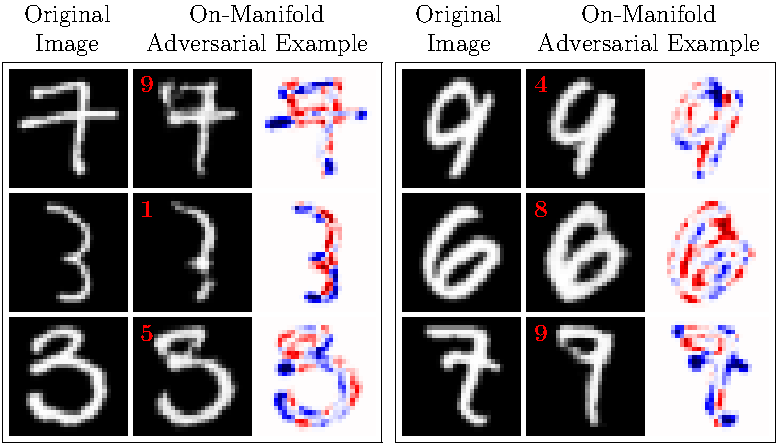
\includegraphics[width=0.45\textwidth]{appendix_data_examples.pdf}
    \caption{On-manifold adversarial examples crafted using class-agnostic \VAEGANs on \MNIST. We show examples illustrating the problematic of unclear class boundaries within the learned manifold. On-manifold adversarial examples are not guaranteed to be label invariant, \ie, they may change the actual, true label according to the approximate data distribution.}
    \label{fig:appendix-data-examples}
\end{figure}
\begin{figure}[t]
    \centering
    \vskip -0.4cm
    \begin{subfigure}{0.235\textwidth}
        \centering
        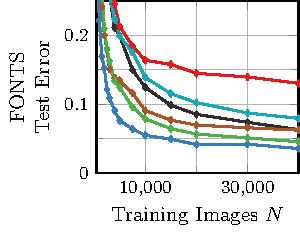
\includegraphics[width=\textwidth]{appendix_data_fonts_error.pdf}
    \end{subfigure}
    \begin{subfigure}{0.235\textwidth}
        \centering
        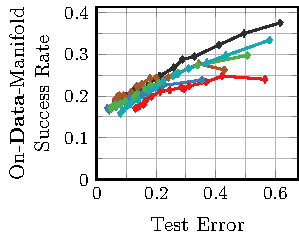
\includegraphics[width=\textwidth]{appendix_data_fonts_error_on_learned.pdf}
    \end{subfigure}
    \\
    \begin{subfigure}{0.235\textwidth}
        \centering
        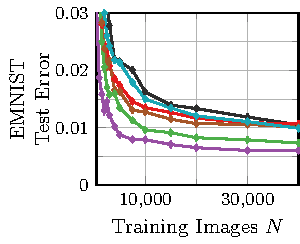
\includegraphics[width=\textwidth]{appendix_data_emnist_error.pdf}
    \end{subfigure}
    \begin{subfigure}{0.235\textwidth}
        \centering
        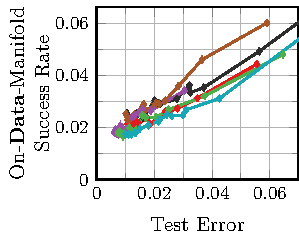
\includegraphics[width=\textwidth]{appendix_data_emnist_error_on_learned.pdf}
    \end{subfigure}
    \\
    \fcolorbox{black!50}{white}{
        \begin{subfigure}{0.45\textwidth}
            \centering
            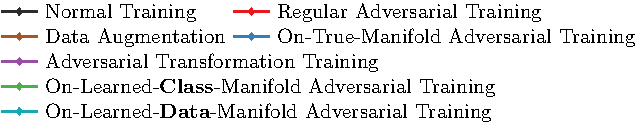
\includegraphics[width=1\textwidth]{appendix_data_legend.pdf}
        \end{subfigure}
    }
    \caption{Test error and on-data-manifold success rate on \Fonts and \MNIST. Using class-agnostic \VAEGANs, without clear class boundaries, on-manifold adversarial training looses its effectiveness -- the on-manifold adversarial examples cross the true class boundaries too often. The strong relationship between on-manifold robustness and generalization can still be confirmed.}
    \label{fig:appendix-data}
\end{figure}

In the context of Sections 3.3 and 3.4 of the main paper, we consider approximating the manifold using class-agnostic \VAEGANs. Instead of the class-conditionals $p(x|y)$ of the data distribution, the marginals $p(x)$ are approximated, \ie, images of different classes are embedded in the same latent space. Then, however, ensuring label invariance, as required by our definition of on-manifold adversarial examples, becomes difficult:
\begin{definition}[On-Manifold Adversarial Example]
    Given the data distribution $p$, an on-manifold adversarial example for $x$ with label $y$ is a perturbed version $\tilde{x}$ such that $f(\tilde{x}) \neq y$ but $p(y|\tilde{x}) > p(y'|\tilde{x}) \forall y' \neq y$.
    \label{def:appendix-on-manifold-adversarial-example}
\end{definition}
\noindent Therefore, we attempt to ensure \defref{def:appendix-on-manifold-adversarial-example} through a particularly small $L_{\infty}$-constraint on the perturbation, specifically $\|\zeta\|_{\infty} \leq \eta$ with $\eta = 0.1$ where $\zeta$ is the perturbation applied in the latent space. Still, as can be seen in \figref{fig:appendix-data-examples}, on-manifold adversarial examples might cross class boundaries, \ie, they change their actual label rendering them invalid according to our definition.

In \figref{fig:appendix-data}, we clearly distinguish between on-\emph{class}-manifold and on-\emph{data}-manifold adversarial training, corresponding to the used class-specific or -agnostic \VAEGANs. Robustness, however, is measured \wrt on-data-manifold adversarial examples.  As can be seen, the positive effect of on-manifold adversarial training diminishes when using on-data-manifold adversarial examples during training. Both, on \Fonts and \MNIST, generalization slightly decreases in comparison to normal training because adversarial examples are not useful for learning the task if label invariance cannot be ensured. When evaluating robustness against on-data-manifold adversarial examples, however, the relation of on-data-manifold robustness to generalization can clearly be seen. Overall, this shows that this relationship also extends to more general, less strict definitions of on-manifold adversarial examples.

\begin{figure}[t]
    \centering
    \vskip -0.4cm
    \begin{subfigure}[t]{0.235\textwidth}
        \centering
        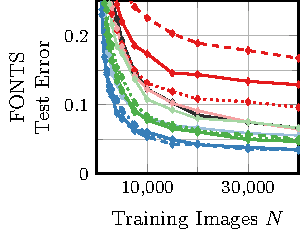
\includegraphics[width=1\textwidth]{appendix_baselines_fonts_error_accuracy.pdf}
    \end{subfigure}
    \begin{subfigure}[t]{0.235\textwidth}
        \centering
        \includegraphics[width=1\textwidth]{appendix_baselines_fonts_error_off_accuracy.pdf}
    \end{subfigure}
    \\
    \begin{subfigure}[t]{0.235\textwidth}
        \centering
        \includegraphics[width=1\textwidth]{appendix_baselines_emnist_error_accuracy.pdf}
    \end{subfigure}
    \begin{subfigure}[t]{0.235\textwidth}
        \centering
        \includegraphics[width=1\textwidth]{appendix_baselines_emnist_error_off_accuracy.pdf}
    \end{subfigure}
    \\
    \fcolorbox{black!50}{white}{
        \begin{subfigure}{0.45\textwidth}
            \centering
            \includegraphics[width=0.7\textwidth]{appendix_baselines_legend.pdf}
        \end{subfigure}
    }
    \vskip -6px
    \caption{Adversarial training variants and baselines on \Fonts and \MNIST. For adversarial training, we consider the  \emph{full variant}, \ie, training on $100\%$ adversarial examples, and the \emph{weak variant}, \ie, stopping the inner optimization problem of \eqnref{eq:appendix-off-manifold-adversarial-training} as son as the first adversarial example is found. For regular adversarial training, the strength of the adversary determines the robustness-generalization trade-off; for on-manifold adversarial training, the ideal strength depends on the approximation quality of the used \VAEGANs.}
    \label{fig:appendix-baselines}
\end{figure}
\begin{figure}[t]
    \centering
    \vskip -0.2cm
    \includegraphics[width=0.4\textwidth]{appendix_tsipras.pdf}
    \vskip -6px
    \caption{Illustration of the toy dataset considered by Tsipras \etal in \cite{TsiprasARXIV2018} and defined in \eqnref{eq:appendix-tsipras}. For labels $y = 1$ and $y = -1$, the two-dimensional observations $x \in \{-1,1\}{\times}\mR$ are plotted. The first dimension, \ie, $x_1$, mirrors the label with probability $0.9$; the second dimension, \ie, $x_2$, is drawn from a Gaussian $\mathcal{N}(y3, I)$, \ie, $\eta$ from the text is $3$. As illustrated on the left, perturbing an observation $x$ with label $y = 1$ but $x_1 = -1$ by $2\eta = 6$ results in an adversarial example $\tilde{x}$ indistinguishable from observations with label $y = -1$.}
    \label{fig:appendix-tsipras}
\end{figure}

\section{Baselines and Adversarial Training Variants}
\label{sec:appendix-adversarian-training}

In the main paper, see Section 3.1, we consider the adversarial training variant by Madry \etal \cite{MadryICLR2018}, \ie,
\vskip -14px
\begin{align}
    \min_w \sum_{n = 1}^N \max_{\|\delta\|_{\infty} \leq \epsilon} \cL(f(x_n + \delta; w), y_n),
    \label{eq:appendix-off-manifold-adversarial-training}
\end{align}
\vskip -4px
\noindent where $f$ is the classifier with weights $w$, $\cL$ is the cross-entropy loss and $x_n$, $y_n$ are training images and labels. In contrast to \cite{MadryICLR2018}, we train on $50\%$ clean and $50\%$ adversarial examples \cite{SzegedyARXIV2013,GoodfellowARXIV2014}. The inner optimization problem is run for full $40$ iterations, as described in \secref{sec:appendix-attacks} without early stopping. Here, we additionally consider the \emph{full variant}, \ie, training on $100\%$ adversarial examples; and the \emph{weak variant}, \ie, stopping the inner optimization problem as soon as the label changes. Additionally, we consider random perturbations as baseline, \ie, choosing the perturbations $\delta$ uniformly at random without any optimization. The same variants and baselines apply to on-manifold adversarial training and adversarial transformation training.

In Section 3.6 of the main paper, we observed that different training strategies might exhibit different robustness-generalization characteristics. For example, regular adversarial training renders the learning problem harder: in addition to the actual task, the network has to learn (seemingly) random but adversarial noise directions leaving the manifold. In \figref{fig:appendix-baselines}, we first show that training on randomly perturbed examples (instead of adversarially perturbed ones) is not effective, neither in image space nor in latent space. This result highlights the difference between random and adversarial noise, as also discussed in \cite{FawziNIPS2016}. For regular adversarial training, the strength of the adversary primarily influences the robustness-generalization trade-off; for example, the weak variant increases generalization while reducing robustness. Note that this effect also depends on the difficulty of the task, \eg, \Fonts is considerably more difficult than \MNIST. For on-manifold adversarial training, in contrast, the different variants have very little effect; generalization is influenced only slightly, while regular robustness is -- as expected -- not influenced.

\section{Definition of Adversarial Examples}
\label{sec:appendix-adversarial-example}

\begin{figure*}[t]
    \centering
    \vskip -0.4cm
    \includegraphics[width=1\textwidth]{appendix_examples_2.pdf}
    \vskip -6px 
    \caption{Regular and on-manifold adversarial examples on \Fonts, \MNIST, \Fashion and \Celeb. On \Fonts, the manifold is known; otherwise, class manifolds have been approximated using \VAEGANs. In addition to the original test images, we also show the adversarial examples and their (normalized) difference (or the magnitude thereof for \Celeb).}
    \label{fig:appendix-examples-2}
\end{figure*}

Adversarial examples are assumed to be label-invariant, \ie, the actual, true label does not change. For images, this is usually enforced using a norm-constraint on the perturbation -- \eg, \cf \eqnref{eq:appendix-off-manifold-madry}; on other modalities, however, this norm-constraint might not be sufficient. In Section 3.3 of the main paper, we provide a definition for on-manifold adversarial examples based on the true, underlying data distribution -- as restated in \defref{def:appendix-on-manifold-adversarial-example}. Here, we use this definition to first discuss a simple and intuitive example before considering the theoretical argument of \cite{TsiprasARXIV2018}, claiming that robust \emph{and} accurate models are not possible on specific datasets; an argument in contradiction to our results

Let the observations $x$ and labels $y$ be drawn from a data distribution $p$, \ie, $x, y \sim p(x, y)$. Then, given a classifier $f$ we define adversarial examples as follows:
\begin{definition}[Adversarial Example]
    Given the data distribution $p$, an adversarial example for $x$ with label $y$ is a perturbed version $\tilde{x}$ such that $f(\tilde{x}) \neq y$ but $p(y|\tilde{x}) > p(y'|\tilde{x}) \forall y' \neq y$.
    \label{def:appendix-adversarial-example}
\end{definition}
\noindent In words, adversarial examples must not change the actual, true label \wrt the data distribution. Note that this definition is identical to \defref{def:appendix-on-manifold-adversarial-example} for on-manifold adversarial examples. For the following toy examples, however, the data distribution has non-zero probability on the whole domain or we only consider adversarial examples $\tilde{x}$ with $p(\tilde{x}) > 0$ such that \defref{def:appendix-adversarial-example} is well-defined. We leave a more general definition of adversarial examples for future work.

We illustrate \defref{def:appendix-adversarial-example} on an intuitive, binary classification task. Specifically, the classes $y = 1$ and $y = -1$ are uniformly distributed, \ie, $p(y = 1) = p(y = -1) = 0.5$ and observations are drawn from point masses on $0$ and $\epsilon$:
\vskip -14px
\begin{align}
p(x = 0|y=1) &= 1\\
p(x = \epsilon|y = -1) &= 1
\end{align}
\vskip -4px
\noindent  This problem is linearly separable for any $\epsilon > 0$; however, it seems that no classifier will be adversarially robust against perturbations of absolute value $\epsilon$. For simplicity, we consider the observation $x = 0$ with $y = 1$ and the adversarial example $\tilde{x} = x + \epsilon = \epsilon$. Then, verifying \defref{def:appendix-adversarial-example} yields a contradiction:
\vskip -14px
\begin{align}
    0 = p(y = 1 | x = \epsilon) \not> p(y = -1 | x = \epsilon) = 1.
\end{align}
\vskip -4px
\noindent  It turns out, $\tilde{x} = \epsilon$ is not a proper adversarial example. This example illustrates that an exact definition of adversarial examples, \eg, \defref{def:appendix-adversarial-example}, is essential to study the robustness of such toy datasets.

\subsection{Discussion of \cite{TsiprasARXIV2018}}

In \cite{TsiprasARXIV2018}, Tsipras \etal argue that there exists an inherent trade-off between regular robustness and generalization based on a slightly more complex toy example; we follow the notation in \cite{TsiprasARXIV2018}. Specifically, for labels $y = 1$ and $y = -1$ with $p(y = 1) = p(y = -1) = 0.5$, the observations $x \in \{-1,1\}{\times}\mR$ are drawn as follows\footnote{Note that, for simplicity and convenience, we consider the $2$-dimensional case; Tsipras \etal consider the general $D$-dimensional case, where $x_1$ remains unchanged and $x_2,\ldots, x_D$ are drawn from the corresponding Gaussian, \cf \eqref{eq:appendix-tsipras}.}:
\vskip -14px
\begin{align}
    \begin{split}
        p(x_1 | y) &= \begin{cases}p & \text{ if }x_1 = y\\1-p & \text{ if }x_1 = -y\end{cases},\\\quad p(x_2 | y) &= \mathcal{N}(x_2; y\eta, 1)
    \end{split}
    \label{eq:appendix-tsipras}
\end{align}
\vskip -4px
\noindent where $\eta$ defines the degree of overlapping between the two classes and $p \geq 0.5$. \figref{fig:appendix-tsipras} illustrates this dataset for $p = 0.9$ and $\eta = 3$. For a $L_{\infty}$-bounded adversary with $\epsilon \geq 2\eta$, Tsipras \etal show that no model can be both accurate and robust. Specifically, for $x$ with $y = 1$ but $x_1 = -1$ and $x_2 = \eta$, we consider replacing $x_2$ with $\tilde{x}_2 = x_2 - 2\eta = -\eta$, as considered in \cite{TsiprasARXIV2018}. However, this adversary does not produce proper adversarial examples according to our definition. Indeed,
\vskip -14px
\begin{align}
    \begin{split}
        p(y = 1 |& x = \tilde{x})\\
        &= p(y = 1 | x_1 = -1) \cdot p(y = 1 | x_2 = - \eta)\\
        &= (1 - p) \cdot \mathcal{N}(x_2 = - \eta; \eta, 1)\\
        &\not> p \cdot \mathcal{N}(x_2 = - \eta; -\eta, 1)\\
        &= p(y = -1 | x_1 = -1) \cdot p(y = -1 | x_2 = - \eta)\\
        &= p(y=-1 | x = \tilde{x})
    \end{split}
\end{align}
\vskip -4px
\noindent which contradicts our definition. Thus, in light of \defref{def:appendix-adversarial-example}, the suggested trade-off of Tsipras \etal is questionable. However, we note that this argument explicitly depends on our definition of proper and invalid adversarial examples, \ie, \defref{def:appendix-adversarial-example}; other definitions of adversarial examples or adversarial robustness, \eg, in the context of the adversarial loss defined in \cite{TsiprasARXIV2018}, may lead to different conclusions.
\end{appendix}
